% Set up the document
\documentclass{article}

% Page size
\usepackage[
    letterpaper,]{geometry}

% Lines between paragraphs
\setlength{\parskip}{\baselineskip}
\setlength{\parindent}{0pt}

% Math
\usepackage{mathtools}
\usepackage{amssymb}
\usepackage{commath}

% Math notation macros
\def\*#1{\mathbf{#1}}
\newcommand{\dadvd}[2]{\dfrac{\text{D} #1}{\text{D} #2}} % advective derivative

\newcommand{\rhat}{\mathbf{\hat{r}}}
\newcommand{\thetahat}{\boldsymbol{\hat{\theta}}}
\newcommand{\xhat}{\mathbf{\hat{x}}}
\newcommand{\yhat}{\mathbf{\hat{y}}}
\newcommand{\zhat}{\mathbf{\hat{z}}}

% Links
\usepackage{hyperref}

% Page numbers at top right
\usepackage{fancyhdr}
\pagestyle{fancy}
\fancyhf{}
\fancyhead[R]{\thepage}
\renewcommand\headrulewidth{0pt}

% Graphics
\usepackage{float}
\usepackage{graphicx}
\graphicspath{ {./img/} }

\begin{document}

\textbf{MATH 462 Assignment 4} \\
\textbf{Matt Wiens \#301294492} \\
\textbf{2020-02-05}

\textbf{A) A Spinning Bucket Problem.}
Consider the steady flow velocity $\*u = (u, v, w) = (-\Omega y, \Omega x,
0)$. Verify that it is an incompressible flow. Explain clearly why it
corresponds to a uniformly rotating fluid (also known as a solid body
rotation). Then use the momentum equation (with gravity $\*F = - \rho g
\zhat$) to solve for the accompanying pressure field $p(x, y, z)$. As a
differential equation problem, explain why the condition $p(0, 0,
0) = p_{atm}$ is sufficient to uniquely determine the pressure.

Now discuss and resolve the apparent confusion suggested in the first
two paragraphs of Problem 1.2 (Acheson) involving the Bernoulli
streamline theorem (Section 1.3). (Extra: Why might an astronomer with
access to a lot of mercury find this result interesting?)

\textbf{Solution}

This flow is incompressible because
%
\begin{equation*}
    \nabla \cdot \*u
        = \dpd{}{x} \del{-\Omega y} + \dpd{}{y} \del{\Omega x} + \dpd{}{z} (0)
        = 0
\end{equation*}
%
where the derivatives vanished because $\Omega$ is a constant and $y$
and $x$ are independent of each other. The flow $\*u$ corresponds to a
uniformly rotating fluid because
%
\begin{equation*}
    \nabla \times \*u
        = \del{
            \dpd{}{x} \del{\Omega x} - \dpd{}{y} \del{- \Omega y}
        } \zhat
        = 2 \Omega \, \zhat
        ;
\end{equation*}
%
that is, the vorticity is constant everywhere and the fluid is rotating
uniformly. Now, the Euler momentum equation tells us that
%
\begin{equation*}
    \dpd{\*u}{t} + (\*u \cdot \nabla) \*u = - \frac{1}{\rho} \nabla p - g \zhat
    .
\end{equation*}
%
Noting that
%
\begin{equation*}
    \dpd{\*u}{t} = \*0; \quad
    (\*u \cdot \nabla) \*u = \del{- \Omega^2 x, - \Omega^2 y, 0}
    ,
\end{equation*}
%
we can solve for the pressure field using the momentum equation by
solving the system
%
\begin{equation*}
    \begin{dcases}
        p_x &= \rho \Omega^2 x \\
        p_y &= \rho \Omega^2 y \\
        p_z &= - \rho g
    \end{dcases}
    .
\end{equation*}
%
This system is simple enough that we can read off the solution
%
\begin{equation*}
    p(x, y, z) = \rho \del{- g z + \frac{\Omega^2 (x^2 + y^2)}{2}} + p_{atm}
    .
\end{equation*}
%
From a mathematical point of view, the $p_{atm}$ term can be any
constant, since the constant vanishes when we take the gradient, and
hence Euler's equations ``work'' no matter what we set the constant to
be. We just need to pick some constant that makes agrees with our
physical interpretation of the system (chosen to be $p_{atm}$ here) and
then each point in space will have a single pressure value associated
with it.

Let's consider the confusion suggested in the Acheson problem. Since our
flow is steady, the quantity
%
\begin{equation*}
    \frac{p}{\rho} + \frac{1}{2} \*u^2 + g z
\end{equation*}
%
is constant along streamlines. According to Acheson, this would
seemingly imply that the constant pressure surfaces take the form
%
\begin{equation*}
    z = \text{constant} - \frac{\Omega^2 (x^2 + y^2)}{2 g}
    .
\end{equation*}
%
The confusion here is that this would imply that the surface of a
rotating bucket of water is at its highest in the center, which goes
against physical intuition (it should be lowest in the center).

One mistake here is that the result only holds along streamlines. It
appears that they are being generalized to all of space in this example.
Additionally, $p$ being constant also implies an extra dependence
between $x$, $y$, and $z$ not considered in the apparent confusion. That
is, if pressure is constant (using our above result) we also have that
%
\begin{equation*}
    z = \text{another constant} + \frac{\Omega^2 (x^2 + y^2)}{2 g}
    .
\end{equation*}
%
Evaluating the conserved quantity using the $p$ we calculated, we have
that
%
\begin{align*}
    H &= \frac{p}{\rho} + \frac{1}{2} \*u^2 + g z \\
      &= - g z + \frac{\Omega^2 (x^2 + y^2)}{2} + \frac{p_{atm}}{\rho}
        + \frac{\Omega^2 (x^2 + y^2)}{2} + g z \\
      &= \Omega^2 (x^2 + y^2) + \frac{p_{atm}}{\rho}
\end{align*}
%
is constant along streamlines, which does not lead to any confusion
regarding rotating buckets.

For the ``extra'' part of this question, I have no idea why an
astronomer with access to lots of mercury would be interested in this
result.

\newpage

\textbf{D) Streamlines \& Streamfunctions.}
The plotting assignment of Homework \#0 involved in the identification
of a streamfunction whose level curves correspond to level streamlines.
This problem explores another example of this idea.

In cylindrical coordinates, an axisymmetric flow has no dependence on
the $\theta$ variable. A Stokes streamfunction, $\Psi(r, z)$, provides a
steady, axisymmetric flow velocity having the form
%
\begin{equation*}
    \*u = U(r, z) \rhat + W(r, z) \zhat
\end{equation*}
%
through the derivative relations
%
\begin{equation*}
    U = - \frac{1}{r} \dpd{\Psi}{z}; \quad W = + \frac{1}{r} \dpd{\Psi}{r}
    .
\end{equation*}

\textbf{i)} For the specific case of the Stokes streamfunction
%
\begin{equation*}
    \Psi(r, z) = \frac{A}{2} r^2 + \frac{m}{4 \pi} \del{1 - \frac{z}{\sqrt{r^2 + z^2}}}
    ,
\end{equation*}
%
compute the velocity components, then verify they satisfy the
incompressibility condition.

\textbf{ii)} Show that this $\Psi(r, z)$ is constant along streamlines
by verifying that
%
\begin{equation*}
    \dadvd{\Psi}{t} = 0
    .
\end{equation*}
%
\textbf{iii)} Show that the flow direction is tangent to the streamline
contours everywhere, and note that the calculation is exactly the same
as in \textbf{ii)}. (Is this a coincidence?)

\textbf{iv)} Use the \texttt{contour} command in Matlab to produce a
graphic illustrating the flow by streamlines and flow direction arrows.
Annotate with parameter values, and all other relevant comments.

\textbf{v)} Find the exact location of the flow stagnation point (where
$\*u = \*0$). What is the value of the streamfunction there? Add this
special contour to your plot, and note that this contour can act as a
separating streamline of the flow (i.e., separating into ``inside'' and
``outside'' parts).

\textbf{vi)} Use the Bernoulli streamline theorem to give a formula for
the pressure deviation (assume that the pressure far upstream is a
constant, $p_{atm}$, and no body forces). Label regions of the
relatively high (H) and/or low (L) pressure regions on your flow graphic
(you may add these by hand, or plot the pressure field as an extra
Matlab plot). Verify that these regions are consistent with the observed
streamline curvatures.

\textbf{vii)} Based on parts \textbf{i)}--\textbf{vi)}, is it clear that
this combination of velocity and pressure fields is a solution to the
incompressible Euler equations? Explain your reasoning.

\newpage

\textbf{Solution}

\textbf{i)} Taking $\Psi$ to be the Stokes streamfunction shown above,
we have that
%
\begin{align*}
    U &= - \frac{1}{r} \dpd{\Psi}{z}
        = \frac{m r}{4 \pi} \frac{1}{\del{r^2 + z^2}^{\frac{3}{2}}}
        , \\
    W &= + \frac{1}{r} \dpd{\Psi}{r}
        = A + \frac{m z}{4 \pi} \frac{1}{\del{r^2 + z^2}^{\frac{3}{2}}}
        .
\end{align*}
%
We can verify the incompressibility condition either by explicitly
computing the divergence or by noting that that mixed partial
derivatives commute. For the latter approach, we have that
%
\begin{equation*}
    \nabla \cdot \*u
        = \frac{1}{r} \dpd{\del{r U}}{r} + \dpd{W}{z}
        = \frac{1}{r} \dpd{}{r} \del{- \dpd{\Psi}{z}}
            + \dpd{}{z} \del{\frac{1}{r} \dpd{\Psi}{r}}
        = - \frac{1}{r} \dmd{\Psi}{2}{r}{}{z}{}
            + \frac{1}{r} \dmd{\Psi}{2}{z}{}{r}{}
        = 0
        .
\end{equation*}
%
\textbf{ii)} Now we will verify that $\Psi$ is constant along
streamlines. In the advective derivative
%
\begin{equation*}
    \dadvd{\Psi}{t} = \dpd{\Psi}{t} + (\*u \cdot \nabla) \Psi
    ,
\end{equation*}
%
the first term vanishes because $\Psi$ does not depend on $t$. The
second term also vanishes, since
%
\begin{equation*}
    (\*u \cdot \nabla) \Psi
        = \del{- \frac{1}{r} \dpd{\Psi}{z}, \frac{1}{r} \dpd{\Psi}{r}}
            \cdot \del{\dpd{\Psi}{r}, \dpd{\Psi}{z}}
        = - \frac{1}{r} \dpd{\Psi}{z} \dpd{\Psi}{r}
            +\frac{1}{r} \dpd{\Psi}{r} \dpd{\Psi}{z}
        = 0
        .
\end{equation*}
%
Therefore we have that
%
\begin{equation*}
    \dadvd{\Psi}{t} = 0
    ,
\end{equation*}
%
and we can conclude that $\Psi$ is constant along streamlines.

\textbf{iii)} To show that the flow direction is tangent to the
streamline contours everywhere, we need to show that $\*u$ is always
orthogonal to $\nabla \Psi$; that is, that $\*u \cdot \nabla \Psi = 0$
everywhere. This calculation is already done in step \textbf{ii)} above,
so we can conclude that the flow direction is indeed tangent to the
stream contours everywhere.

We saw in Homework 0 that the flow followed the streamline contours, so
this result should be expected.

\textbf{iv)} The plot below shows level curves of $\Psi$ (coloured),
along with a quiver plot of the velocity field $\*u$. Note that some of
the velocity quivers near the center of the plot were removed, since,
relatively speaking, these quivers were too large, which made the other
quivers to hard to see. As is displayed in the title of the plot, the
values of the constants used are $A = 20$ and $m = 100$.

Also displayed is the point where $\*u = 0$ with a red star, along with
the associated contour in black (see part \textbf{v)}).

\textbf{v)} To find the point where $\*u = 0$ we need both $U = 0$ and $W =
0$. Here we will assume that in general both $A$ and $m$ are non-zero.
In order to have $U = 0$, we clearly need $r = 0$. Given that $r = 0$, if
$W = 0$, we can find the required $z$ by solving
%
\begin{equation*}
    A + \frac{m z}{4 \pi} \frac{1}{\del{z^2}^{3/2}} = 0
\end{equation*}
%
which gives us that $z = - \frac{\text{sgn}(A)}{2} \sqrt{\frac{m}{|A|
\pi}}$, where sgn gives the sign of its argument. The value of $\Psi$ at
this point is $\Psi = \frac{m}{2 \pi}$.

This contour at this value of $\Psi$ appears to be a ``separating''
streamline, since the behaviour on either side of the contour is very
different. Inside of this region, there is a clear source of flow, where
the flow velocity is very high close to the source. Outside of the
region the flow seems to be moving past the region.

\textbf{vi)} Since we have a steady flow, the quantity
%
\begin{equation*}
    H = \frac{p}{\rho} + \frac{1}{2} \*u^2
\end{equation*}
%
is conserved along streamlines. Solving for pressure, we have that
%
\begin{equation*}
    p = p_{atm} - \frac{\rho}{2} \del{\*u^2 - A^2}
    .
\end{equation*}
%
where the constant was chosen such that $p = p_{atm}$ when $r$ or $z$
get large, since as either $r$ or $z$ get large in magnitude, $\*u^2 \to
A^2$.

The pressure is plotted with the center bit taken out (there is
extremely negative pressure in the middle). The result is quite
unintuitive. In the inner region, flow seems to be going against the
pressure gradient, which doesn't really make sense to me. On the outer
region the pressure appears to be consistent with the streamline.

\textbf{vii)} Judging from the plots alone, outside of the middle
region, the fluid appears well behaved and appears to satisfy the
incompressible Euler equations. However, inside of this region,
the flow appears extremely divergent, and hence does not appear to
satisfy the incompressible Euler equations.

For the extra part of this problem, outside of the ``inside'' of the
separating streamline, the flow reminds me of waters' flow when a
ship or submarine moves through it.

\newpage

\begin{figure}
    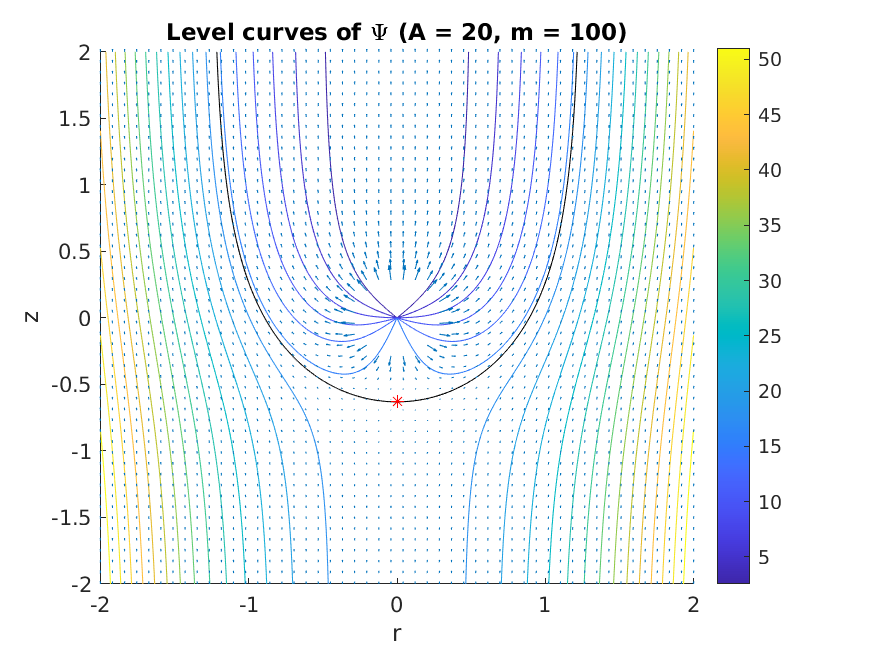
\includegraphics[width=\textwidth]{fig1}
    \centering
\end{figure}

\newpage

\begin{figure}
    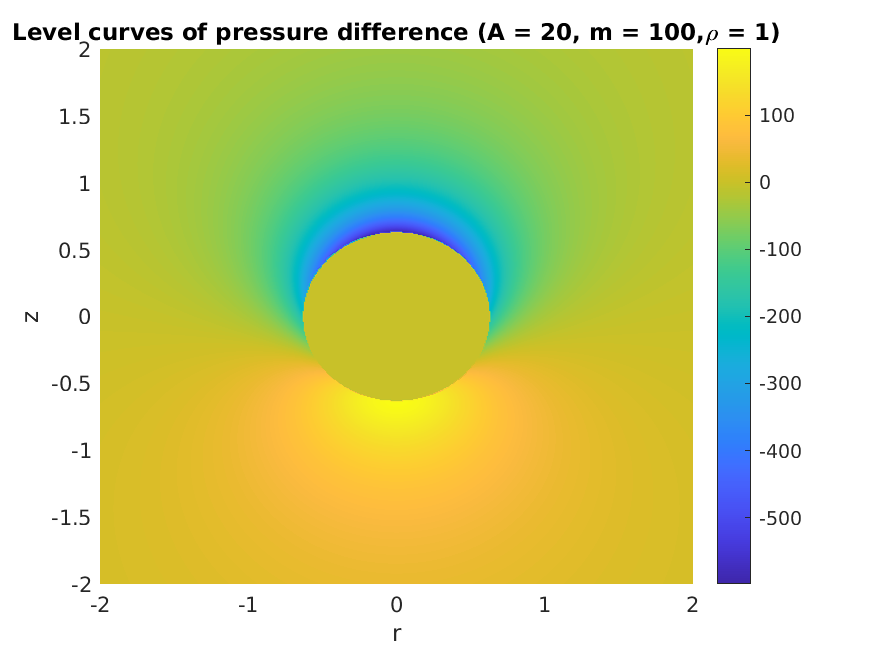
\includegraphics[width=\textwidth]{fig2}
    \centering
\end{figure}

\end{document}
